\documentclass[a4paper,12pt]{scrartcl}
\usepackage[utf8x]{inputenc}
\usepackage[T1]{fontenc} % avec T1 comme option  d'encodage c'est ben mieux, surtout pour taper du français.
%\usepackage{lmodern,textcomp} % fortement conseillé pour les pdf. On peut mettre autre chose : kpfonts, fourier,...
\usepackage[french]{babel} %Sans ça les guillemets, amarchpo
\usepackage{amsmath}
\usepackage{multicol}
\usepackage{amssymb}
\usepackage{tkz-tab}
\usepackage{exercice_sheet}

%\trait
%\section*{}
%\exo{}
%\question{}
%\subquestion{}

\date{}


% Title Page
\title{Devoir maison 1, CG-2, corrigé}

\author{Mathématiques}

\begin{document}

\maketitle

\exo{Équations, inéquations}

Résoudre les équations et inéquations suivantes.

\question{}
$\ln(x+1) + \ln(x-2) = \ln(18)$

Attention aux ensembles de définition des logarithmes. On doit d'abord tenir compte du fait que leurs arguments (ici $x+2$ et $x-2$ doivent être \emph{strictement positifs}):

$x+1 > 0$ soit $x > -1$ d'une part, et $x-2 > 0$ soit $x>2$ d'autre part. Ainsi, toutes les solutions qui ne seront pas strictement supérieures à 2 ne devront pas faire partie de la réponse. 

On peut donc écrire: 

$\ln(x+1) + \ln(x-2) = \ln(18)$

$\Leftrightarrow (x+1)(x-2) = 18$ pour $x > 2$.

$\Leftrightarrow x^2 - x - 20 = 0$

$\Delta = 1 + 4 \times 20 = 81$ d'où $\sqrt{\Delta} = 9$

$x_1 = \dfrac{1 - 9}{2} = -4$ et 
$x_2 = \dfrac{1 + 9}{2} = 5$

Mais comme -4 est hors des ensembles de définitions de $\ln(x+1)$ et $\ln(x-2)$, seul 5 doit être pris en compte.

$$S = \left\lbrace 5 \right\rbrace$$

\question{}
$2e^{2t} + 9e^t = 5$

Remarque: contrairement à ci-dessus, les exponentielles sont définies sur $\mathbb{R}$, il n'y a donc pas de contrainte sur l'ensemble de définition.

Changement de variable : on pose $X = e^t$.

On obtient le polynôme suivant: $2X^2 + 9X - 5 = 0$. 

$\Delta = 81 + 4 \times 2 \times 5 = 121$ donc $\sqrt{\Delta} = 11$.

$X_1 = \dfrac{-9 - 11}{4} = -5$ et 
$X_2 = \dfrac{-9 + 11}{4} = \dfrac{1}{2}$

\littlestar{$X_1 = -5$}

On a donc $e^{t_1} = X_1 = -5$. Une exponentielle étant toujours strictement positive, $X_1$ n'apporte pas de solution à l'équation. Autrement dit, il n'existe pas de valeur de $t_1$ telle que $e^{t_1} = -5$.

\littlestar{$X_2 = \dfrac{1}{2}$}

$e^{t_2} = X_2 = \dfrac{1}{2}$
$\Leftrightarrow t_2 = \ln \dfrac{1}{2} = - \ln 2$

L'unique solution  de cette équation est donc $- \ln 2$. On a donc:

$$S = \left\lbrace - \ln 2 \right\rbrace$$

\question{}
$2e^{2t} - 9e^t + 4 = 0$

De la même façon, on obtient: $2X^2 - 9X + 4 = 0$.

$\Delta = 81 - 4 \times 2 \times  4 = 49$, donc $\sqrt{\Delta} = 7$.

$X_1 = \dfrac{9 - 7}{4} = \dfrac{1}{2}$ et 
$X_2 = \dfrac{9 + 7}{4} = 4$.

On a donc $e^{t_1} = \dfrac{1}{2}$ soit $t_1 = -\ln 2$

et $e^{t_2} = 4$ soit $t_2 = \ln 4 = 2 \ln 2$

$$S = \left\lbrace -\ln 2 ; 2 \ln 2 \right\rbrace$$



\question{}
$\ln(x^4) < 12$

Ensemble de définition: $x^4 > 0 \Leftrightarrow x \neq 0$.

$\Leftrightarrow e^{\ln x^4} < e^{12}$

$\Leftrightarrow x^4 < e^{12}$

On rappelle que pour une inéquation du type $x^2 < k$, l'ensemble des solutions est $S = \left[ -\sqrt{k} ; \sqrt{k} \right]$

Ainsi:

$\Leftrightarrow -e^{6} < x^2 < e^{6}$

$\Leftrightarrow -e^{3} < x < e^{3}$.

On doit enlever 0 de l'ensemble des solutions. On obtient donc:

$$S = \left[ -e^{3} ; 0 \right[ \cup \left] 0 ; e^{3} \right]$$.

Que l'on eut également écrire $S = \left[ -e^{3} ; e^{3} \right] - \left\lbrace 0 \right\rbrace$.


\exo{Suites numériques}

\question{Justifier que le nombre d'élèves de l'école B pour l'année $2015+n$ peut être modélisé par une suite géométrique $(b_n)$ dont on précisera le premier terme $b_0$ et la raison $q$.}

D'une année sur l'autre, l'effectif est augmenté de 5\%, donc \textbf{multiplié} par 1.05. Il s'agit là de la raison $q$ de la suite, qui est géométrique. L'année 2015 correspond à l'année initiale. L'effectif en 2015 correspond à 280 élèves, et il n'agit du premier terme $b_0$. 

La suite $\left( b_n \right)$ a donc pour raison $q = 1.05$ et $b_0 = 280$.

\question{La capacité de l'école B est de 450 élèves. Pourra-t-elle accueillir tous les élèves prévus par le modèle jusqu'en 2025?}

D'après le résultat de la question précédente, le terme général de la suite $\left( b_n \right)$ est: $b_n = 280 \times 1.05^n$. 

L'année 2025 correspond au rang $n = 10$. On doit donc calculer $b_{10}$. 

$b_{10} = 280 \times 1.05^{10} \approx 456$ (arrondi à l'entier le plus proche). 

Conclusion: ça va être chaud pour l'école B en 2025.

\question{}
Dans le tableur ci-dessous, quelle formule dois-je écrire dans la cellule C3 pour calculer l'effectif de l'école A? 

Il faut taper \texttt{=C2+10}.

Même question pour la cellule D3, qui concerne l'école B.

De même: \texttt{=D2*1.05}.

Que faire pour que les colonnes entières soient calculées sans avoir à taper la formule dans chaque case de chaque colonne?

Il faut tirer la poignée de la cellule vers le bas afin de recopier la formule.

\begin{center}
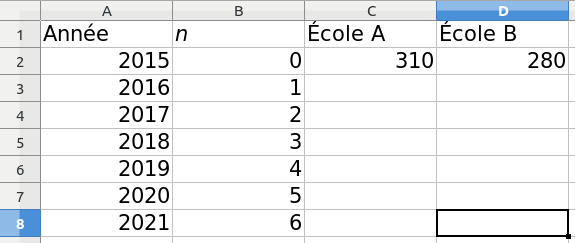
\includegraphics[width=0.5\textwidth]{pics/1.png}
\end{center}

\exo{Étude d'une fonction}

On considère la fonction $f$ définie sur $[0;+\infty[$ par:

$$f(x) = 0.4 e^{0.3x}$$

On désigne par $C$ sa courbe représentative dans un repère orthogonal et par $f'$ sa fonction dérivée. Unités graphiques: 1cm pour une unité sur l'axe des abscisses et 1cm pour 2 unités sur l'axe des ordonnées.

\question{Étudier la limite\footnote{Les limites ne sont pas au programme pour les suites mais le sont pour les fonctions.} de $f$ en $+\infty$.}

$\lim\limits_{x\to+\infty} 0.3 x = +\infty$

D'où $\lim\limits_{x\to+\infty} e^{0.3 x} = +\infty$.

Et donc $\lim\limits_{x\to+\infty} 0.4 e^{0.3 x} = +\infty$.

Soit $\lim\limits_{x\to+\infty} f(x) = +\infty$


\question{Étude de la fonction}

\subquestion{Calculer $f'(x)$}

$f'(x) = 0.4 \times 0.3 e^{0.3 x} = 0.12 e^{0. x}$.

\subquestion{Étudier le signe de $f'(x)$ et donner le tableau de variation de $f$ sur $[0;+\infty[$.}

$e^{0.3 x} > 0, \forall x \in \mathbb{R}$. Multiplier par 0.4 ne change pas le signe, on a donc $f'(x) > 0, \forall x \in [0 : +\infty[$.

\begin{center}
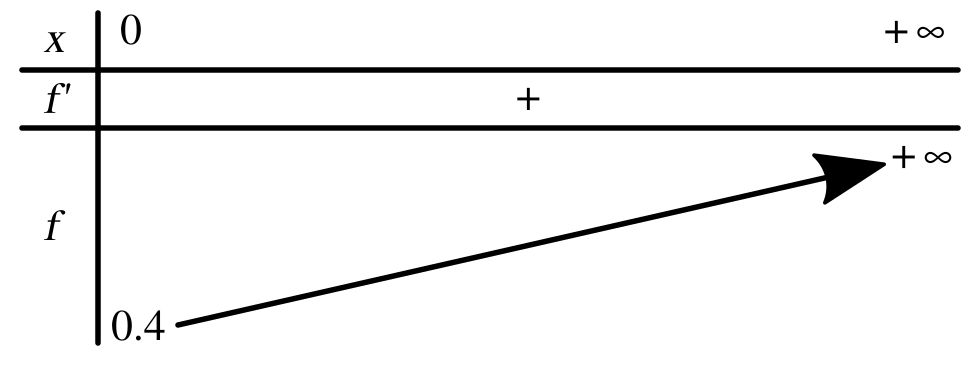
\includegraphics[width=0.5\textwidth]{pics/2.png}
\end{center}



\subquestion{Tracer $C$. Une feuille à petit carreaux fera parfaitement l'affaire.}

\begin{center}
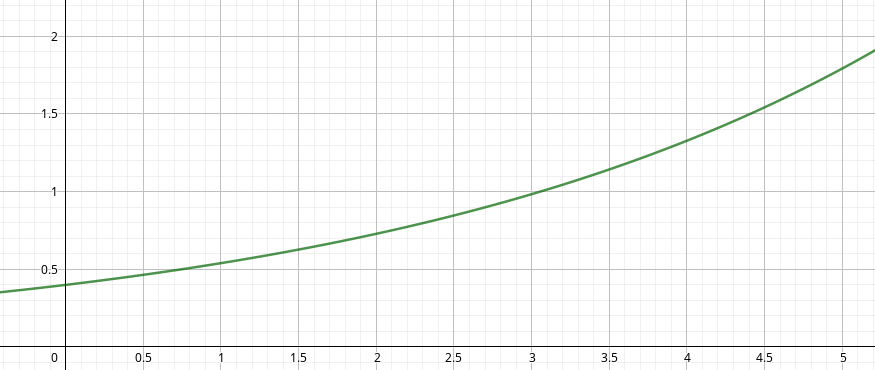
\includegraphics[width=1\textwidth]{pics/3.png}
\end{center}

\trait

\begin{center}
Fin.
\end{center}

\end{document}
